A set $R=\{r_1, r_2, r_3 \}$ of robots  is deployed in the environment graphically described in  Fig.~\ref{fig:example1}.
This environment represents a building made by four rooms $L=\{ l_1, l_2, l_3, l_4 \}$, which has been affected by an earthquake.
The environment is further partitioned in cells, each labeled with an identifier in $c_1, c_2, \ldots, c_{30}$.
Robots $r_1$, $r_2$, and $r_3$ are placed in their initial locations.
Each robot is able to move from one cell to another, by performing action $mov$.
The robots are also able to perform the following actions.
Robot $r_1$ is able to load debris of the building by performing action $ld$. 
In Fig.~\ref{fig:example1} the cells in which a robot $r$ can perform an action $\alpha$ are marked with the label $r(\alpha)$.
Robot $r_2$ can wait until another robot loads debris on it by performing action $rd$ and can unload debris by performing one of the two actions $ud1$ and $ud2$. 
Actions $ud1$ and $ud2$ use different actuators.
Specifically, action $ud1$ uses a gripper while action $ud2$ exploits a dump mechanism.
Robot $r_3$ is able to take pictures by performing action $tp$ and send them using a communication network through the execution of action $sp$. 
Symbols $r_1(ld)$, $r_2(rd)$, $r_2(ud1)$, $r_2(ud2)$, $r_3(tp)$, and $r_3(sp)$ are used in Fig.~\ref{fig:example1} to mark the regions where  actions can be executed by the robots, while movement actions are not reported for graphical reasons.
Each action may be associated with a service, which is a high-level functionality provided by the robot when an action is performed.
For example, actions $ld$, $rd$, $tp$, and $sp$  are associated with the services \emph{load\_carrier}, \emph{detect\_load}, \emph{take\_snapshot}, and \emph{send\_info}, respectively.
Actions $ud1$ and $ud2$ are associated with service \emph{unload}.
The labels $L(\pi,\alpha)=\trueval$ below Fig.~\ref{fig:example1} are used to indicate that a service $\pi$ is associated with  action $\alpha$. 
Robots must meet and  synchronously execute actions. 
In this example, robots $r_1$ and  $r_2$ must meet  in cell $c_7$ and synchronously execute actions $ld$ and $rd$, respectively. 
The cells where meeting is requested are marked with rotating arrows marked with the identifiers of the robots that must meet, meaning that, in order to meet, the robots must be on the same cell to meet.


\begin{figure}[!t]
\begin{center}
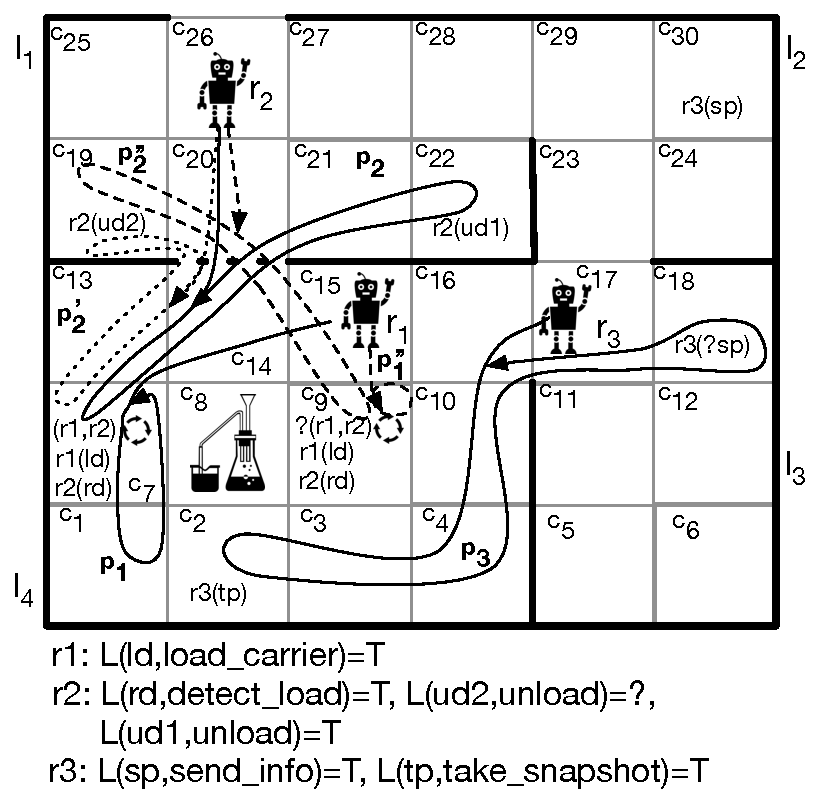
\includegraphics[width=0.9\linewidth]{Figures/motivatingExample.pdf}
\caption{An example showing the model of the robots and their environment. Plans computed by \toolName\ are represented by trajectories marked with arrows.}
\label{fig:example1}
\end{center}
\end{figure}

The \emph{mission}  the team of robots has to achieve is to check whether toxic chemicals have been released by the container located in $l_4$.
We assume that the mission is specified through a set of \emph{local missions} assigned to each robot of the team and described in Linear Time Temporal Logic  (LTL).
An LTL formula is obtained by composing actions with standard LTL operators: $\Next$ (next), $\Event$  (eventually),  $\Always$ (always) and $\Until$ (until)~\cite{pnueli1977temporal}. 
In our example the mission  can be specified by means of the following local missions: $\phi_1=\Always (\Event ($\emph{load\_carrier}$))$, 
$\phi_2=\Always (\Event($\emph{detect\_ load} $ \wedge \Event ($\emph{unload}$)))$, 
 $\phi_3=\Always ( \Event ($\emph{take\_snapshot} $\wedge \Event ($\emph{send\_info}$)))$, which are assigned to robot $r_1$, $r_2$ and $r_3$, respectively.
The formulae specify that periodically robot $r_1$ loads debris on $r_2$ (by performing action \emph{load\_carrier}), robot $r_2$ receives debris (when action \emph{detect\_ load} occurs)  and brings them to an appropriate unload area (by performing action \emph{unload}), and robot $r_3$ continuously takes pictures (by performing action \emph{take\_snapshot}) and sends them using the communication network (by performing action \emph{send\_info}).
Informally, while $r_3$ continuously takes pictures and sends them using the communication network, $r_1$ and $r_2$ remove debris to allow $r_3$ having a better view on the container.
The pictures allow verifying whether toxic chemicals have been released by the container.

The presence of partial knowledge about the robots and their environment is described in the following.

\textbf{Partial knowledge about the actions execution.} 
The robots can move between cells separated by grey lines, while they cannot cross black bold lines.
It is unknown whether it is possible to move between cells $c_{14}$ and $c_{20}$ since the structure may have been affected by collapses.
This is indicated using a dashed black bold line.
It is also unknown whether robot $r_3$ can send pictures using a communication network in location $l_3$ and specifically in cell $c_{18}$, i.e., whether action $s_p$ can be performed. 
Locations of the environment where it is unknown if an action can be provided are marked with the name of the action preceded by symbol $?$.

\textbf{Unknown service provisioning.} 
There are cases in which actions can be executed but there is uncertainty about service provisions.
For example, actions $ud1$ and $ud2$ of robot $r_2$ unload the robot.
Action $ud2$ will always be able to provide the \emph{unload} service, while it is unknown whether $ud1$ is actually able to provide this service since its effectiveness depends on the size of the collected debris. 
 In Fig.~\ref{fig:example1}, the label $L(ud1,unload)=?$ indicates that there is partial knowledge  about the provision of the \emph{unload} service when action $ud1$ is performed. 

\textbf{Unknown meeting capabilities.} 
It is  unknown whether robots $r_1$ and $r_2$ can meet in one cell of the environment. 
For example, a collapse in the roof of the building may forbid the two robots to concurrently execute services $ld$ and $rd$, i.e., there is not enough space for $r1$ to load $r2$. 
Unknown meeting capabilities are indicated with rotating arrows labeled with the symbol $?$.
For example,  in Fig.~\ref{fig:example1}, it is unknown whether robots $r_1$ and $r_2$ are able to meet in cell $c_{9}$.


